
\chapter{Observer}

\section{Allgemein}
Das Observer Design Pattern (Beobachter Entwurfsmuster) gehört zu der Kategorie der behavioural 
patterns (Verhaltensmuster). Es wird verwendet, um die Änderung an dem Zustandes eines Objekts zu
erfassen und alle davon abhängigen Objekte über die Änderung automatisch zu
informieren.\\
\newline
Die Funktionsweise des Observer Design Patterns erfordert zwei Arten von Objekten. Das Subject 
stellt Daten zur Verfügung und arbeitet fortlaufend mit diesen. Wurden diese Daten verändert
informiert das Subject seine Observer und teilt ihnen mit, das sich der Objektzustand verändert 
hat. Der Observer kann anschließend auf diese Zustandsänderung reagieren.\\
\newline
Ein Beispiel für diesen Anwendungsfall ist eine grafische Oberfläche, welche Daten anzeigt 
die sich im laufenden Betrieb ändern können. Die grafische Oberfläche ist der Observer und die 
Klasse, welche die Daten zur Verfügung stellt ist das Subject. Sobald sich nun Daten ändern, 
wird der Observer vom Subject informiert und dieser kann anschließend die Daten auf der 
grafischen Oberfläche aktualisieren.\\
\newline

\begin{figure}[!htbp]
	\centering
	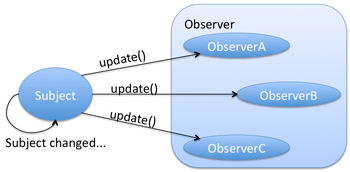
\includegraphics[width=0.66\textwidth]{content/pictures/Observer/observer01.png}
	\label{pic:bild}
	\caption{Observer Diagramm \cite{paulObserver}}
\end{figure}

Es gibt drei verschiedene Arten um diese Funktionalität umzusetzen, wobei jede ihre Vor- und 
Nachteile hat.\\ 
\newline
Push Notification\\
Bei der Push Notification benachrichtigen die Subjects ihre Observer nur dahingehend, das 
sich etwas an dem Objektzustand verändert hat, aber nicht was für eine Veränderung das ist. 
Dadurch ist dies die schnellste Variante.\\
\newline
Push-Update Notification\\
Bei dieser Art der Umsetzung wird zusätzlich zu der Information über die Zustandsänderung
auch noch die geänderten Daten mitübertragen.\\
\newline
Pull Notification\\
Bei der Pull Notification informieren nicht die Subjects die Observer sondern die Observer 
fragen in regelmäßigen Abstand bei den Subjects nach, ob Änderungen vorliegen. Aufgrund des 
regelmäßigen Abfragens wird diese Variante seltener verwendet als die beiden anderen, da hier 
deutlich mehr Rechenzeit von der Observerfunktion benötigt wird.\\
\newline
Ein Nachteil des Observer Patterns ist der hohe Aufwand bei Änderungen am
Subject. Hier muss dann auch der Observer angepasst werden, was hohe Änderungskosten zur
Folge hat.\cite{wikiObserver}\\\\
Aufgrund der höheren Flexibilität wollen wir eine Push-Notification zum Einsatz bringen.

 \begin{lstlisting}
class Subject {
public:
    void register_Observer(
    	shared_ptr<Observer> observer) = 0;
    void delete_Observer(
    	shared_ptr<Observer> observer) = 0;
    void notify_Observer() = 0;
};
 
class ConcreteSubjekt : public Subject {
    vector<shared_ptr<Observer>> _observer;
    int   _value;
public:
    ConcreteSubjekt() : _value(0) {}
 
    void register_Observer(
    	shared_ptr<Observer> observer) {
    	
        _observer.add(observer);
    }
    void delete_Observer(shared_ptr<Observer>
    	observer) {
    	
        auto pos = find_if(_observer.begin(), _observer.end(),
        	 [&](shared_ptr<Observer> const& b) { 
        	 	return *b == *observer;
         });
          
         if (pos != _observer.end()) 
         	_observer.erase(pos);
    }
    void notify_Observer() {
        for (auto& beo : _observer) {
            beo->update(_value);
        }
    }
 
    void setValue(int value) {
        _value = value;
        notify_Observer();
    }
};
 
class Observer {
public:
	void update(){
	
	}
};
 
class ConcreteObserver1 : public Observer {
public:
    void update() {
        out << "Observer 1\n";
    }
};
 
class ConcreteObserver2 : public Observer {
public:
    void update(int value) {
        out << "Observer 2\n";
    }
};
 
int main() {
    shared_ptr<Subject> oneSubject(new KonkretesSubjekt());
    shared_ptr<Observer> observer1(
    		new ConcreteObserver1());
    shared_ptr<Observer> observer2(
    		new ConcreteObserver2());
 
    oneSubject->register_Observer(observer1);
    oneSubject->register_Observer(observer2);
 
    oneSubject->setValue(10);
    oneSubject->delete_Observer(observer1);
    oneSubject->setValue(20);
}
\end{lstlisting}

\section{Umsetzung}

Für die Umsetzung des Observer Design Pattern in Rhapsody wurden einige Richtlinien und 
Implementierungsdetails ausgearbeitet.\\
\newline
Für das Observer Design Pattern stehen zwei Stereotypen zur Verfügung. Zum einen der Observer 
und zum anderen das Subject. Wenn eine Klasse als Stereotyp Observer deklariert wird, wird das 
zugehörige Interface erstellt und in das bestehende Projekt eingefügt, mit dem Stereotyp Subject 
wird ebenso verfahren.\\
\newline
Um eine fehlerfreie Umsetzung zu realisieren wurde festgelegt, das ein Benutzer im Lauf seiner 
Softwareentwicklung keine reservierten Klassen- und Methodennamen benutzen darf. So dürfen 
keine Klassen existieren die Observer oder Subject heißen. Darüber hinaus dürfen auch keine 
Methoden aus diesen zwei Interfaces vom Benutzer manuell im Voraus implementiert werden. 
Diese Richtlinien werden bei der Übersetzung des Programms überprüft und im Fehlerfall 
entsprechende Fehlermeldungen generiert und die Übersetzung abgebrochen.\\
\newline
Das Observer Interface besitzt lediglich eine Methode update, welche als leere Methode 
implementiert wird. Das hat den Hintergrund, dass nicht ersichtlich ist wie auf Änderungen 
reagiert werden soll. Die Funktionalität muss vom Benutzer selbst festgelegt und implementiert 
werden.\\
\newline
Das Subject Interface besitzt drei öffentliche Methoden. Mit der Methode register_Observer 
können Observer für dieses Subject in eine Liste hinzugefügt werden, und mit delete_Observer 
wieder entfernt. Diese zwei Methoden werden vom Interface automatisch vollständig zur Verfügung
gestellt. Die Methode notify_Observer wird leer implementiert, da der Benutzer über die 
Funktionalität selbst entscheiden muss, zum Beispiel welche Attribute überwacht werden 
sollen und welche nicht.\\
\newline
Wird dieses Design Pattern verwendet, ist es zwar durchaus möglich, dass ein Benutzer ein 
Observer ohne ein Subject implementiert oder umgekehrt. Jedoch macht die Verwendung 
dieser Stereotypen nur gemeinsam einen Sinn. In solch einem Fall soll das Programm zwar 
übersetzt werden, aber dennoch eine Warnung ausgegeben werden um den Benutzer darauf hinzuweisen.

						